\documentclass{article}
\usepackage[utf8]{inputenc}
\usepackage{titling}
\usepackage{natbib}
\usepackage{graphicx}
\usepackage{enumitem}
\usepackage{varwidth}
\usepackage{tikz}
\usetikzlibrary{matrix,calc}
\graphicspath{ {./images/} }

\setlength{\droptitle}{-10em}

\title{Combinational Logic: Binary-to-Seven-Segment Decoder}
\author{Ezra John Guia
        30031697}
\date{February 8^{th}, 2019}

\begin{document}

\maketitle

\section*{Design Method}

\begin{enumerate}[label=\arabic*]

%%%%%%%%%%%%%%%%%%%%%%% DM 1 %%%%%%%%%%%%%%%%%%%%%%%
    \item State the problem in words
    \vspace{1 mm}
    
    Design a combinational logic circuit that takes a 4-bit binary number as an input and produces 7 outputs, one each for the 7 segments of the display unit to show the corresponding hexadecimal number.
    
%%%%%%%%%%%%%%%%%%%%%%% DM 2 %%%%%%%%%%%%%%%%%%%%%%%
    \vspace{3 mm}
    \item Determine the input and output variables
    \vspace{1 mm}
    
    \begin{varwidth}[t]{.5\textwidth}
        4-bit Input variables:
        \begin{itemize}
            \item bit - 3 (w)
            \item bit - 2 (x)
            \item bit - 1 (y)
            \item bit - 0 (z)
        \end{itemize}
    \end{varwidth}
        \hspace{4em}
    \begin{varwidth}[t]{.5\textwidth}
        Output variables:
        \begin{itemize}
            \item A
            \item B
            \item C
            \item D
            \item E
            \item F
            \item G
        \end{itemize}
    \end{varwidth}
    
%%%%%%%%%%%%%%%%%%%%%%% DM 3 %%%%%%%%%%%%%%%%%%%%%%%
    %\newpage
    \vspace{3 mm}
    \item Assign letter symbols to the variables.
    \vspace{1 mm}
    
    The 4-bit input variables will be represented by w, x, y, z respectively.
    
    
%%%%%%%%%%%%%%%%%%%%%%% DM 4 %%%%%%%%%%%%%%%%%%%%%%%
    \newpage
    %\vspace{3 mm}
    \item Create the truth table that defines the relationships between inputs and outputs. \\
    %%\vspace{3 mm}
    
    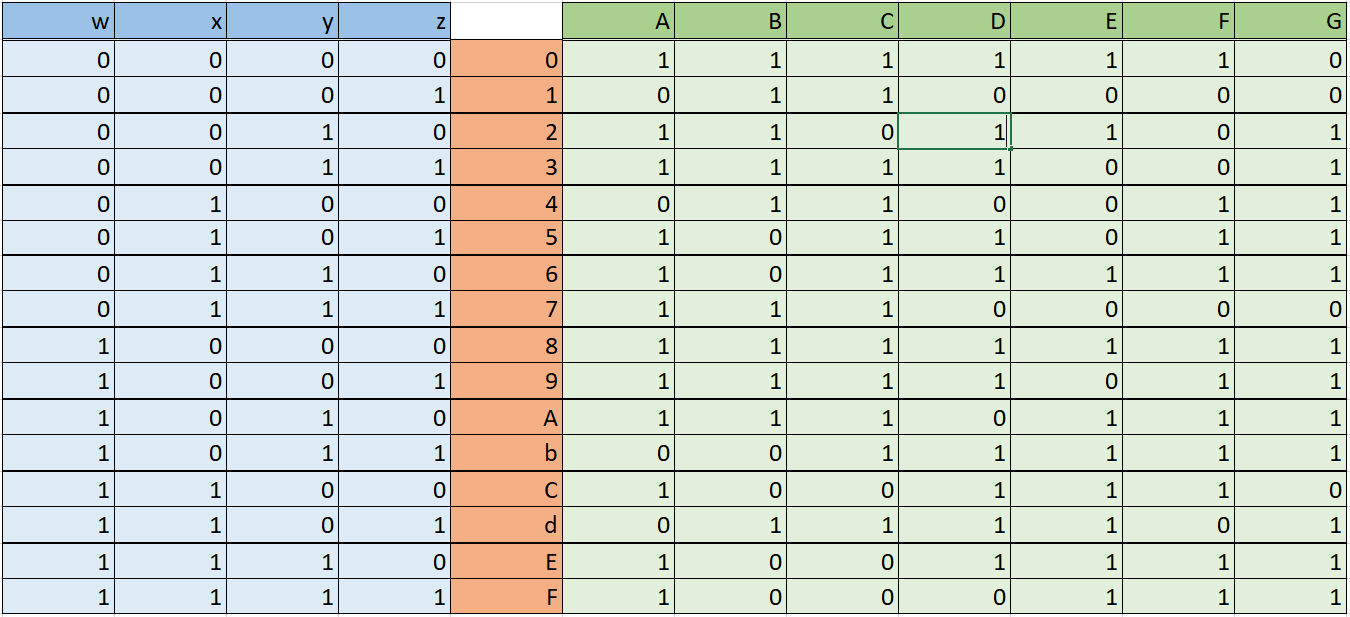
\includegraphics[scale=0.325]{TruthTable.PNG}

%%%%%%%%%%%%%%%%%%%%%%% DM 5 %%%%%%%%%%%%%%%%%%%%%%%
    \vspace{3 mm}
    \item Obtain the simplified function for each output (show all steps for this, whether done algebraically or using the map method). \\
    %%\vspace{3 mm}

%%%%%%%%%%%%%%%%%%%%%%% K-MAP CODE

    %isolated term
    %#1 - Optional. Space between node and grouping line. Default=0
    %#2 - node
    %#3 - filling color
    \newcommand{\implicantsol}[3][0]{
        \draw[rounded corners=3pt] ($(#2.north west)+(135:#1)$) rectangle ($(#2.south east)+(-45:#1)$);
    }

    %internal group
    %#1 - Optional. Space between node and grouping line. Default=0
    %#2 - top left node
    %#3 - bottom right node
    %#4 - filling color
    \newcommand{\implicant}[4][0]{
        \draw[rounded corners=3pt] ($(#2.north west)+(135:#1)$) rectangle ($(#3.south east)+(-45:#1)$);
        }

    %group lateral borders
    %#1 - Optional. Space between node and grouping line. Default=0
    %#2 - top left node
    %#3 - bottom right node
    %#4 - filling color
    \newcommand{\implicantcostats}[4][0]{
        \draw[rounded corners=3pt] ($(rf.east |- #2.north)+(90:#1)$)-| ($(#2.east)+(0:#1)$) |- ($(rf.east |- #3.south)+(-90:#1)$);
        \draw[rounded corners=3pt] ($(cf.west |- #2.north)+(90:#1)$) -| ($(#3.west)+(180:#1)$) |- ($(cf.west |- #3.south)+(-90:#1)$);
    }

    %group top-bottom borders
    %#1 - Optional. Space between node and grouping line. Default=0
    %#2 - top left node
    %#3 - bottom right node
    %#4 - filling color
    \newcommand{\implicantdaltbaix}[4][0]{
        \draw[rounded corners=3pt] ($(cf.south -| #2.west)+(180:#1)$) |- ($(#2.south)+(-90:#1)$) -| ($(cf.south -| #3.east)+(0:#1)$);
        \draw[rounded corners=3pt] ($(rf.north -| #2.west)+(180:#1)$) |- ($(#3.north)+(90:#1)$) -| ($(rf.north -| #3.east)+(0:#1)$);
    }

    %group corners
    %#1 - Optional. Space between node and grouping line. Default=0
    %#2 - filling color
    \newcommand{\implicantcantons}[2][0]{
        \draw[rounded corners=3pt] ($(rf.east |- 0.south)+(-90:#1)$) -| ($(0.east |- cf.south)+(0:#1)$);
        \draw[rounded corners=3pt] ($(rf.east |- 8.north)+(90:#1)$) -| ($(8.east |- rf.north)+(0:#1)$);
        \draw[rounded corners=3pt] ($(cf.west |- 2.south)+(-90:#1)$) -| ($(2.west |- cf.south)+(180:#1)$);
        \draw[rounded corners=3pt] ($(cf.west |- 10.north)+(90:#1)$) -| ($(10.west |- rf.north)+(180:#1)$);}

    %Empty Karnaugh map 4x4
    \newenvironment{Karnaugh}%
    {
    \begin{tikzpicture}[baseline=(current bounding box.north),scale=0.8]
    \draw (0,0) grid (4,4);
    \draw (0,4) -- node [pos=0.7,above right,anchor=south west] {yz} node [pos=0.7,below left,anchor=north east] {wx} ++(135:1);
    %
    \matrix (mapa) [matrix of nodes,
            column sep={0.8cm,between origins},
            row sep={0.8cm,between origins},
            every node/.style={minimum size=0.3mm},
            anchor=8.center,
            ampersand replacement=\&] at (0.5,0.5)
    {
                           \& |(c00)| 00         \& |(c01)| 01         \& |(c11)| 11         \& |(c10)| 10         \& |(cf)| \phantom{00} \\
    |(r00)| 00             \& |(0)|  \phantom{0} \& |(1)|  \phantom{0} \& |(3)|  \phantom{0} \& |(2)|  \phantom{0} \&                     \\
    |(r01)| 01             \& |(4)|  \phantom{0} \& |(5)|  \phantom{0} \& |(7)|  \phantom{0} \& |(6)|  \phantom{0} \&                     \\
    |(r11)| 11             \& |(12)| \phantom{0} \& |(13)| \phantom{0} \& |(15)| \phantom{0} \& |(14)| \phantom{0} \&                     \\
    |(r10)| 10             \& |(8)|  \phantom{0} \& |(9)|  \phantom{0} \& |(11)| \phantom{0} \& |(10)| \phantom{0} \&                     \\
    |(rf) | \phantom{00}   \&                    \&                    \&                    \&                    \&                     \\
    };
    }%
    {
    \end{tikzpicture}
    }

    %Defines 8 or 16 values (0,1,X)
    \newcommand{\contingut}[1]{%
    \foreach \x [count=\xi from 0]  in {#1}
         \path (\xi) node {\x};
    }
    
    %Places 1 in listed positions
    \newcommand{\minterms}[1]{%
        \foreach \x in {#1}
            \path (\x) node {1};
    }
    
    %Places 0 in listed positions
    \newcommand{\maxterms}[1]{%
        \foreach \x in {#1}
            \path (\x) node {0};
    }
    
    %Places X in listed positions
    \newcommand{\indeterminats}[1]{%
        \foreach \x in {#1}
            \path (\x) node {X};
    }
    
%%%%%%%%%%%%%%%%%%%%%%% K-MAP CODE END

%%%%%%%%%%%%%%%%%%%%%%% A
    \textbf{Karnaugh Map for A}
    
    \begin{Karnaugh}
        \contingut{1,0,1,1,0,1,1,1,1,1,1,0,1,0,1,1}
        \implicantcostats{12}{10}{white} % wz'
        \implicantcantons[2pt]{white} % x'z'
        \implicant{8}{9}{white} % wx'y'
        \implicant{5}{7}{white} % w'xz
        \implicant{3}{6}{white} % w'y
        \implicant{7}{14}{white} % xy
    \end{Karnaugh}
    
    A = wz' + x'z' + wx'y' + w'xz + w'y + xy
    
    \newpage

%%%%%%%%%%%%%%%%%%%%%%% B
    \textbf{Karnaugh Map for B}
    
    \begin{Karnaugh}
        \contingut{1,1,1,1,1,0,0,1,1,1,1,0,0,1,0,0}
        \implicantcantons[2pt]{white} % x'z'
        \implicant{0}{2}{white} % w'x'
        \implicant{0}{4}{white} % w'y'z'
        \implicant{3}{7}{white} % w'yz
        \implicant{13}{9}{white} % wy'z
    \end{Karnaugh}
    
    B = x'z' + w'x' + w'y'z' + w'yz + wy'z
    
    \vspace{2mm}
%%%%%%%%%%%%%%%%%%%%%%% C
    \textbf{Karnaugh Map for C}
    
    \begin{Karnaugh}
        \contingut{1,1,0,1,1,1,1,1,1,1,1,1,0,1,0,0}
        \implicant{1}{9}{white} % y'z
        \implicant{8}{10}{white} % wx'
        \implicant{4}{6}{white} % w'x
        \implicant{0}{5}{white} % w'y'
        \implicant{1}{7}{white} % w'z
    \end{Karnaugh}
    
    C = y'z + wx' + w'x + w'y' + w'z
    
    \vspace{2mm}
%%%%%%%%%%%%%%%%%%%%%%% D
    \textbf{Karnaugh Map for D}
    
    \begin{Karnaugh}
        \contingut{1,0,1,1,0,1,1,0,1,1,0,1,1,1,1,0}
        \implicant{12}{9}{white} % wy'
        \implicantdaltbaix[3pt]{3}{11}{white} % x'yz
        \implicant{5}{13}{white} % xy'z
        \implicantcostats{0}{2}{white} % w'x'z'
        \implicant{6}{14}{white} % xyz'
    \end{Karnaugh}
    
    D = wy'+ x'yz + xy'z + w'x'z' + xyz'
    
    %\vspace{2mm}
%%%%%%%%%%%%%%%%%%%%%%% E
    \textbf{Karnaugh Map for E}
    
    \begin{Karnaugh}
        \contingut{1,0,1,0,0,0,1,0,1,0,1,1,1,1,1,1}
        \implicantcantons[2pt]{white} % x'z'
        \implicant{2}{10}{white} % yz'
        \implicant{12}{14}{white} % wx
        \implicant{15}{10}{white} % wy
    \end{Karnaugh}
    
    E = x'z' + yz' + wx + wy
    
    \vspace{2mm}
%%%%%%%%%%%%%%%%%%%%%%% F
    \textbf{Karnaugh Map for F}
    
    \begin{Karnaugh}
        \contingut{1,0,0,0,1,1,1,0,1,1,1,1,1,0,1,1}
        \implicant{8}{10}{white} % wx'
        \implicantcostats{4}{14}{white} % xz'
        \implicant{15}{10}{white} % wy
        \implicant{0}{8}{white} % y'z'
        \implicant{4}{5}{white} % w'xy'
    \end{Karnaugh}
    
    F = wx' + xz' + wy + y'z' + w'xy'
    
    \vspace{2mm}
%%%%%%%%%%%%%%%%%%%%%%% G
    \textbf{Karnaugh Map for G}
    
    \begin{Karnaugh}
        \contingut{0,0,1,1,1,1,1,0,1,1,1,1,0,1,1,1}
        \implicantdaltbaix[3pt]{3}{10}{white} % x'y
        \implicant{8}{10}{white} % wx'
        \implicant{2}{10}{white} % yz'
        \implicant{13}{11}{white} % wz
        \implicant{4}{5}{white} % w'xy'
    \end{Karnaugh}
    
    G = x'y + wx' + yz' + wz + w'xy'

%%%%%%%%%%%%%%%%%%%%%%% DM 6 %%%%%%%%%%%%%%%%%%%%%%%
    \vspace{3 mm}
    \item Implement the functions using the appropriate gates (show a logic diagram for this).
    \vspace{1 mm}

    \textbf{Logic Diagram for A} \\
    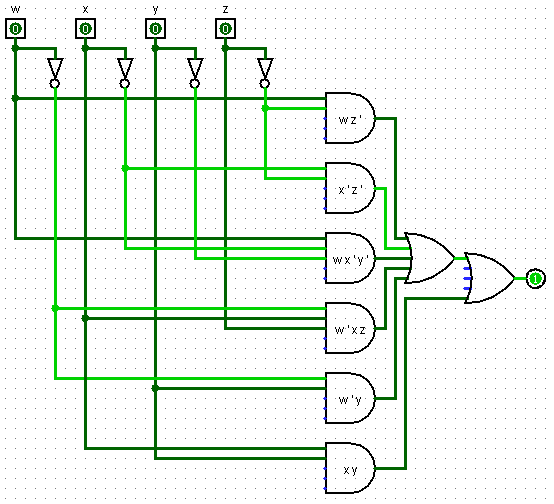
\includegraphics[scale=.72]{A.PNG} \\
    \newpage
    \textbf{Logic Diagram for B} \\
    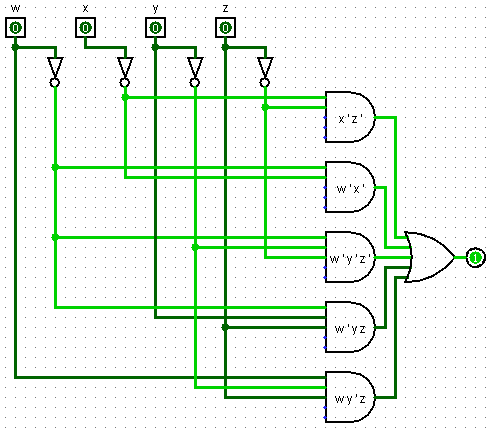
\includegraphics[scale=.72]{B.PNG} \\
    \hfill
    \textbf{Logic Diagram for C} \\
    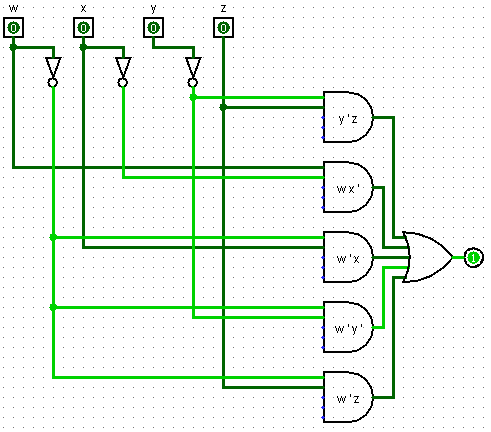
\includegraphics[scale=.72]{C.PNG} \\
    \newpage
    \textbf{Logic Diagram for D} \\
    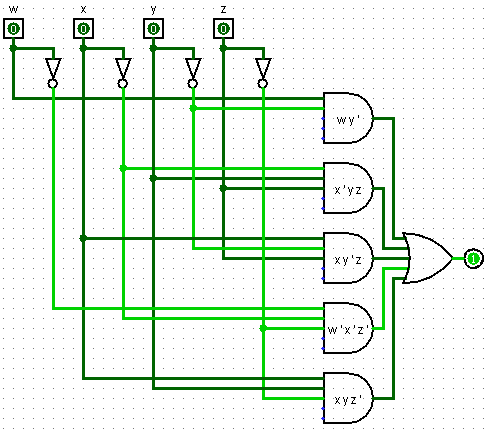
\includegraphics[scale=.72]{D.PNG} \\
    \hfill
    \textbf{Logic Diagram for E} \\
    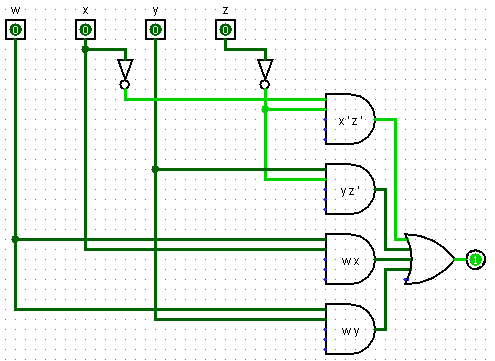
\includegraphics[scale=.72]{E.PNG} \\
    \newpage
    \textbf{Logic Diagram for F} \\
    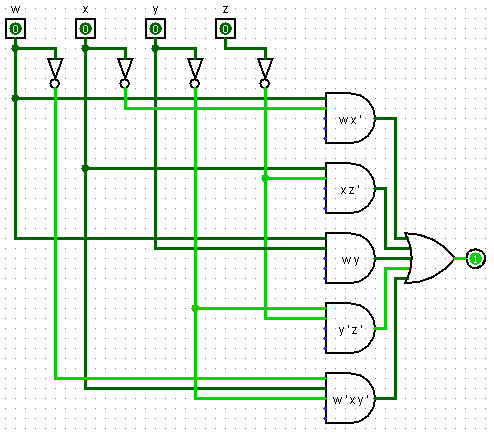
\includegraphics[scale=.72]{F.PNG} \\
    \hfill
    \textbf{Logic Diagram for G} \\
    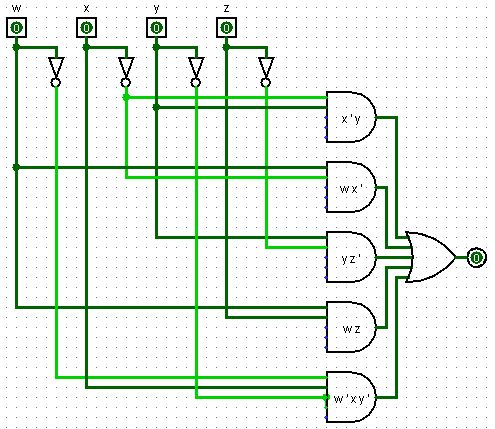
\includegraphics[scale=.72]{G.PNG} \\
    
    %\includegraphics[scale=.72]{LogicDiagram.PNG}


\end{enumerate}
\end{document}